We first identify a set of runtime errors that we would like to detect:

\begin{itemize}
	\itemsep0em
	\item[--] Because of references subtraction, one could try to access the memory with a strictly negative address.
	\item[-] A variable may be used before it is initialized, which could lead to undefined behavior.
	\item[--] If we wish to add the division operator, we may want to detect divisions by zero.
\end{itemize}

We now focus on the first error: invalid memory addresses.
We give an abstract domain for detecting such errors as well as a static analysis, which we then apply to some examples.
Regarding the other errors mentioned, we give later an overview of similar strategies that we could employ to detect them.

\subsection*{Strictly negative memory addresses}

We define the lattice $\mathcal{L} = (E, \subset, \sqcup, \sqcap)$ as illustrated in \figurename~\ref{fig:lattice} to approximate the domain range of the variable values.

\begin{figure}
	\centering
	\begin{tikzpicture}[node distance=2cm]
		\node (Z) at (0,0) {$\mathbb{Z}$};
		\node[below left of=Z] (ZP) {$\mathbb{Z}^{+}$};
		\node[below right of=Z] (ZM) {$\mathbb{Z}^{-}$};
		\node[below left of=ZP] (ZPS) {$\mathbb{Z}^{+*}$};
		\node[below right of=ZM] (ZMS) {$\mathbb{Z}^{-*}$};
		\node[below right of=ZPS] (P1) {$\lbrace 1 \rbrace$};
		\node[left of=P1] (P2) {$\lbrace 2 \rbrace$};
		\node[left of=P2] (P3) {$\ldots$};
		\node[below left of=ZMS] (N1) {$\lbrace -1 \rbrace$};
		\node[right of=N1] (N2) {$\lbrace -2 \rbrace$};
		\node[right of=N2] (N3) {$\ldots$};
		\node[below left of=ZM] (ZE) {$\lbrace 0 \rbrace$};
		\node[below right of=P1] (N) {$\bot_{int}$};
		\draw[-] (Z) -- (ZP) -- (ZPS) -- (P1) -- (N) -- (N1) -- (ZMS) -- (ZM) -- (Z) (ZE) -- (ZP) (N) -- (ZE) -- (ZM) (ZPS) -- (P2) -- (N) -- (N2) -- (ZMS);
		\draw[-] (ZPS) -- (P3) -- (N) -- (N3) -- (ZMS);
	\end{tikzpicture}
	\caption{Abstract domain for detecting invalid memory addresses}
	\label{fig:lattice}
\end{figure}

We now define our static analysis.
At each program point, we define a dictionary that gives an approximation domain for each numerical variable: $\alpha: \var{} \longrightarrow E$.
This dictionary has a finite definition set, which is handy.
For this reason, we do not consider memory values that we simply abstract to the domain $\mathbb{Z}$ since the number of valid addresses is infinite.

If we have context $\Gamma$ and a program $c$ such that $\Gamma \vdash c$, then we define $\alpha^0$ with respects to $\Gamma$:
if $x: \Int \in \Gamma$ then $\alpha^0(x) = \mathbb{Z}$ and if $x: \Ref \in \Gamma$ then $\alpha^0(x) = \mathbb{Z}^{+}$.

For each program point, we now define an \emph{in} and \emph{out} analysis using the control flow graph of the program $c$ as follows:

\[
\forall x \in \var{} \quad \alpha_{in}^l(x) =
	\begin{cases}
		\alpha^0(x) & \text{if $l = init(c)$} \\
		\bigsqcup\limits_{l' \rightarrow l} \alpha_{out}^{l'}(x) & \text{otherwise} \\
	\end{cases}
\]

We now define $\alpha_{out}$ in function of $\alpha_{in}$ for the basic instructions that are not captured by the control flow graph.
We use an approximation function $f: \exp{} \times (\var{} \longrightarrow E) \longrightarrow E$ that we define more precisely further below.

\begin{itemize}
	\itemsep0em
	\item[--] $\left[\texttt{skip}\right]^l$: For all $x$: $\alpha_{out}^l(x) = \alpha_{in}^l(x)$
	\item[--] $\left[x := e\right]^l$: For all $y \neq x$: $\alpha_{out}^l(y) = \alpha_{in}^l(y)$
	
	For x: $\alpha_{out}^l(x) \mapsto f(e, \alpha_{in}^l)$
	\item[--] $\left[[e_1] := e_2\right]^l$: If $f(e_1, \alpha_{in}^l)$ gives an error, we return an error.
	
	Otherwise, for all $x$: $\alpha_{out}^l(x) = \alpha_{in}^l(x)$
\end{itemize}

The function $f$ approximates the domain of the expression depending on the domains of its components and is defined as one would intuitively imagine.
A few examples are given in \tablename~\ref{tab:approx}.

\begin{table}
	\centering
	\begin{tabular}{@{}p{0.15\textwidth}p{0.3\textwidth}p{0.3\textwidth}p{0.15\textwidth}@{}}
	\toprule
	Expressions & Cases 1 & Cases 2 & Output \\
	\midrule
	$x$ & & & $\alpha_{in}^l(x)$ \\
	\midrule
	$n$ & & & $\lbrace \N{}(n) \rbrace$ \\
	\midrule
	$e_1 + e_2$ & if $f(e_1, \alpha_{in}^l) = \mathbb{Z}^{+}$ & if $f(e_2, \alpha_{in}^l) = \mathbb{Z}^{+*}$ & $\mathbb{Z}^{+*}$ \\
	& if $f(e_1, \alpha_{in}^l) = \mathbb{Z}^{+}$ & if $f(e_2, \alpha_{in}^l) = \mathbb{Z}^{-}$ & $\mathbb{Z}$ \\
	& if $f(e_1, \alpha_{in}^l) = \lbrace x \rbrace$ & if $f(e_2, \alpha_{in}^l) = \lbrace y \rbrace$ & $\lbrace x + y \rbrace$ \\
	\midrule
	$e_1 - e_2$ & if $f(e_1, \alpha_{in}^l) = \mathbb{Z}^{-*}$ & if $f(e_2, \alpha_{in}^l) = \mathbb{Z}^{+}$ & $\mathbb{Z}^{-*}$ \\
	& if $f(e_1, \alpha_{in}^l) = \mathbb{Z}^{+}$ & if $f(e_2, \alpha_{in}^l) = \mathbb{Z}^{+}$ & $\mathbb{Z}$ \\
	& if $f(e_1, \alpha_{in}^l) = \lbrace x \rbrace$ & if $f(e_2, \alpha_{in}^l) = \lbrace y \rbrace$ & $\lbrace x - y \rbrace$ \\
	\midrule
	$e_1 \times e_2$ & if $f(e_1, \alpha_{in}^l) = \mathbb{Z}^{-*}$ & if $f(e_2, \alpha_{in}^l) = \mathbb{Z}^{-*}$ & $\mathbb{Z}^{+*}$ \\
	& if $f(e_1, \alpha_{in}^l) = \mathbb{Z}$ & if $f(e_2, \alpha_{in}^l) = \lbrace 0 \rbrace$ & $\lbrace 0 \rbrace$ \\
	& if $f(e_1, \alpha_{in}^l) = \lbrace x \rbrace$ & if $f(e_2, \alpha_{in}^l) = \lbrace y \rbrace$ & $\lbrace x \times y \rbrace$ \\
	\midrule
	$[e]$ & if $f(e, \alpha_{in}^l) = \mathbb{Z}^{+}$ & & $\mathbb{Z}$ \\
	& if $f(e, \alpha_{in}^l) = \mathbb{Z}$ & & Error \\
	& if $f(e, \alpha_{in}^l) = \mathbb{Z}^{-*}$ & & Error \\
	& if $f(e, \alpha_{in}^l) = \lbrace x \rbrace \wedge x < 0$ & & Error \\
	\bottomrule
	\end{tabular}
	\caption{Approximation function $f$: a few examples}
	\label{tab:approx}
\end{table}

\paragraph{Examples}

We consider the following program: $x:= 1; y:= [x]$.
The static analysis is quite trivial and returns no error as expected.
However, if we consider the following program: $x:= 1 - 2; y:= [x]$, we have the following static analysis:

\begin{align*}
	& \alpha_{in}^1 = \lbrace x: \mathbb{Z}^{+}, y: \mathbb{Z} \rbrace & \alpha_{out}^1 = \lbrace x: \lbrace -1 \rbrace, y: \mathbb{Z} \rbrace \\
	& \alpha_{in}^2 = \lbrace x: \lbrace -1 \rbrace, y: \mathbb{Z} \rbrace & \alpha_{out}^2 \longrightarrow \text{Error} \\
\end{align*}

We obtain an error which is satisfying since the program would indeed try to use an invalid memory address.
We can notice that the program $x:= 2 - 1; y:= [x]$ would pass the analysis since we would get $\alpha_{in}^2 = \lbrace x: \lbrace 1 \rbrace, y: \mathbb{Z} \rbrace$ in the send, which is fine.
However, we can still have some valid programs that fail the analysis when loops are involved\todo{explanations}.
With this static analysis, we get some false negative and discard valid programs but we are sure all memory addresses are valid when no error is returned, \ie{} we get an over-estimation of valid programs regarding this type of errors.
 

\section*{Improvements}

\subsection*{Analysing Memory values}
All memory values are approximated by the domain $\mathbb{Z}$.
We could be more precise by considering another function $\beta: E \longrightarrow E$ that would give a domain approximation for the value located in a range of memory addresses.
We would need to adapt the rule for $\left[[e_1] := e_2\right]^l$ where we currently do not use $f(e_2, \alpha_{in}^l)$.


\subsection*{Using the guards}
One can notice that our simple static analysis does not use the guards of the \texttt{if} and \texttt{while} statements. One could use a simple lattice with $\top_{bool}, \lbrace \texttt{true} \rbrace, \lbrace \texttt{false} \rbrace, \bot_{bool}$ to abstract boolean values. This would capture new information, as \texttt{if b then $c_1$ else $c_2$} can be simplified to $c_1$ if \texttt{b} is abstracted by $\lbrace \texttt{true} \rbrace$.
Similarly, \texttt{while b do c} can be simplified to $\texttt{skip}$ if \texttt{b} is abstracted by $\lbrace \texttt{false} \rbrace$.
We then would be more precise and sometimes be able to discard branches that we are actually sure they will not be executed.
For instance, the following program, detected currently as invalid, would pass the static analysis: $\texttt{if true then~} x:= [5] \texttt{~else~} x:= [1 - 2]$.

\subsection*{Uninitialized variables}

So far, programs that use unitialized variables are still well-typed. Our progress theorem states that such programs will still progress if the initial configuration $(\sigma,\delta)$ contains values of the right type.

One could decide to forbid such programs. To do so, one could do a simple static analysis associating a set of declared variables to each program point. Each assignment adds a variable to the set of declared variable. After merging two control flow paths the set of defined variable is the intersection. Using the value of an unitialized variable would raise an error. Of course, this analysis admits some false positives (as in the program \texttt{if true then x:=0 else skip; [0] := x;}) but its success guarantees that each variable has been initialized. 

\subsection*{Division by zero}

One could also desire to add the division to integer arithmetics. Of course, programs using division by 0 would have blocking semantics. Our abstract domains would be enough to detect these cases. Dividing by a value in $\mathbb{Z}, \mathbb{Z^+}, \mathbb{Z^-}$ or $\lbrace 0 \rbrace$ would raise an error. Of course, there are still false alarms, as in \texttt{x := 3 - 2; y := 2 / x;}.


\section*{Summary}

\todo{mini text}

  \begin{center}
    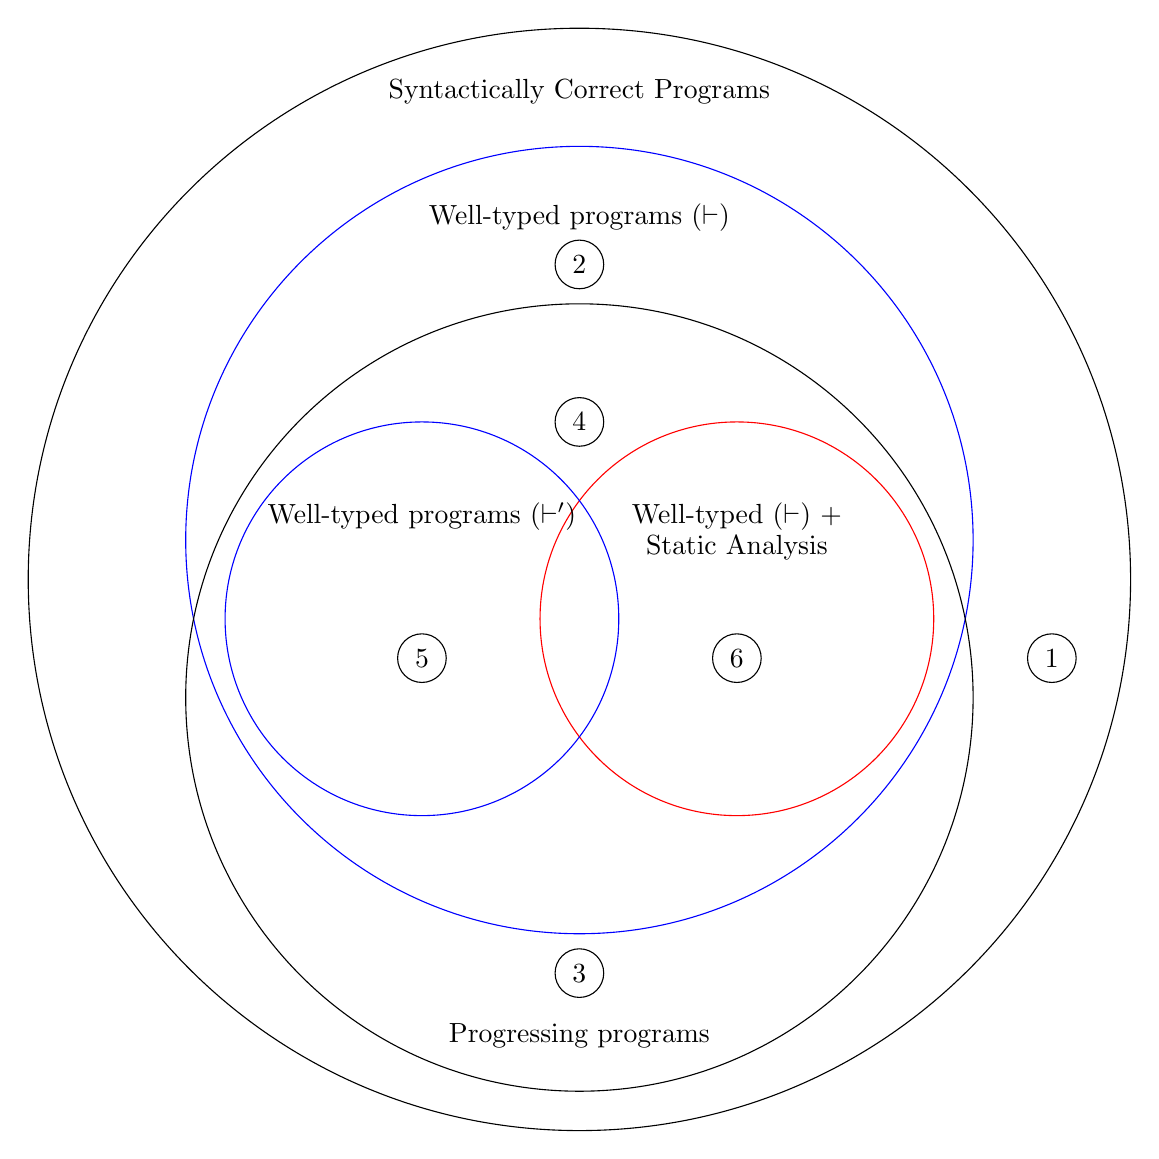
\begin{tikzpicture}[scale=1]
      \draw [color=red](2,0.5) circle (2.5cm);
      \draw [color=blue](0,1.5) circle (5cm);
      \draw (0,-0.5) circle (5cm);
      \draw (0,1) circle (7cm);
      \draw [color=blue] (-2,0.5) circle (2.5cm);
      \node[] at (-2,1.8) {Well-typed programs ($\vdash'$)};
      \node[] at (0,5.6) {Well-typed programs ($\vdash$)};
      \node[] at (0,7.2) {Syntactically Correct Programs};
      \node[] at (0,-4.8) {Progressing programs};
      \node[] at (2,1.8) {Well-typed ($\vdash$) +};
      \node[] at (2,1.4) {Static Analysis};
      \node[circle,draw] at (6,0) {1};
      \node[circle,draw] at (0,5) {2};
      \node[circle,draw] at (0,-4) {3};
      \node[circle,draw] at (0,3) {4};
      \node[circle,draw] at (-2,0) {5};
      \node[circle,draw] at (2,0) {6};
    \end{tikzpicture}
  \end{center}

  
  \paragraph{1:}
  \texttt{x := [-3];}

  \paragraph{2:}
  \texttt{x := [1 - 3];}

  \paragraph{3:}
  \texttt{x := true; x := 1;}

  \paragraph{4:}
  \texttt{x := [3 - 1];}

  \paragraph{5:}
  \texttt{[2] := 3; x := [2]; y := [x];}

  \paragraph{6:}
  \texttt{x := [3 - 0];}
    
